%_____________________________________________________________________________________________ 
% LATEX Template: Department of Comp/IT BTech Project Reports
% Main Report
% Sun Apr 1 20:40:00 IST 2011
% 
%_____________________________________________________________________________________________ 

\documentclass[a4paper,12pt,onecolumn]{report}

%_____________________________________________________________________________________________ 
% Inclusion of Required Packages
%_____________________________________________________________________________________________ 
\usepackage[dvips]{graphics}
\usepackage{color}
\usepackage{epsfig,float}
%_____________________________________________________________________________________________ 
% Page Layout
%_____________________________________________________________________________________________

 \usepackage[left=2.5cm,top=2cm,right=2cm,bottom=2cm,bindingoffset=0.5cm]{geometry}

%\usepackage{geometry}
%\geometry{a4paper,left=35mm,right=20mm,top=20mm,bottom=20mm}
\setlength{\textwidth}{6.5in}
\setlength{\textheight}{10in}
\setlength{\topmargin}{0.0in}
\setlength{\oddsidemargin}{0.0in}			% Customisable
\setlength{\headheight}{0.0in}
\setlength{\headsep}{0.0in}
\setlength{\topskip}{0.0in}
%_____________________________________________________________________________________________ 
% Font Definition
%_____________________________________________________________________________________________ 
\fontencoding{T1}		% Font specification : Times New Roman, Bold, Normal, 18
\fontfamily{cmr}		% Roman
\fontseries{m}			% Medium
\fontshape{n}			% Upright
\fontsize{14pt}{5}		
\linespread{1.5}		% Vertical spacing between lines
\selectfont			% Select the specified font
%_____________________________________________________________________________________________ 
% Main report starts here
%_____________________________________________________________________________________________ 

\begin{document}	% Start of Report
%_____________________________________________________________________________________________ 
%\pagestyle{empty}
%_____________________________________________________________________________________________ 
% Title page: Specifies a custom-made title page
%_____________________________________________________________________________________________ 
\DeclareGraphicsExtensions{.png, .ps}
\begin{titlepage}
\begin{center}
\LARGE{\bf{QUIZ GENERATION CHATBOT\\}}	% LARGE = 17.28
%\vspace{10pt}
\Large{\bf{A Project Report\\}}		% Large = 14.40
\Large{\em{Submitted by\\}}
\begin{table}[htbp]
	\begin{center}
	\begin{tabular}{ l c c l }
	\Large\bf{Vivek R. Bhave} & & & \Large\bf{111508015} \\[0.3cm] 
	\Large\bf{Shreyansh R. Gopawar} & & & \Large\bf{111508073} \\[0.3cm]
	\Large\bf{Aditya D. Neralkar} & & & \Large\bf{111508076} \\
	\end{tabular}
	\end{center}
	\end{table}
\Large{\em{in partial fulfillment for the award of the degree\\ \vspace{1.5pt}of\\}}
\LARGE{\bf{Information Technology\\}}% Mention only appropriate degree.
%\vspace{10pt}
%names of advisors
\Large{Under the guidance of\\ }
\Large{\bf{Dr. Y. V. Haribhakta}\\}
\Large{College of Engineering, Pune\\}
%\vspace{8pt}
% this is applicable only if you have a company based project
%\large{\bf{AND}\\}	% Case changed from full uppercase. Different from doc template. Looks better
%\vspace{10pt}
%\Large{\bf{Mr. Amit Kumar Singh}\\}
%\Large{Hindustan Naturals, Inc.\\}
%\vspace{5pt}
%coep logo added
%\begin{figure}[h]
%\centering
%
\includegraphics[width=3cm,height=3cm]{coeplogo.eps}
%\end{figure}
\Large{\bf{DEPARTMENT OF COMPUTER ENGINEERING AND \\INFORMATION TECHNOLOGY,\\ 
COLLEGE OF ENGINEERING, PUNE-5}}
\vfill
\large{April, 2019}
\end{center}
\end{titlepage}

%\maketitle			% *Generate* the defined title. No definition - no gereration

%_____________________________________________________________________________________________ 
% LATEX Template: Department of Comp/IT BTech Project Reports
% Certificate Page
% Sun Mar 27 10:25:35 IST 2011
% 
% Note: UK English spellings used. 
%_____________________________________________________________________________________________ 
\thispagestyle{empty}
\linespread{2}
\begin{center}			% LARGE = 18
	\Large{\bf{DEPARTMENT OF COMPUTER ENGINEERING AND\\  INFORMATION TECHNOLOGY,\\ 
	       COLLEGE OF ENGINEERING, PUNE\\}}	
\end{center}

\vspace{20pt}			% Vertical space between dept name and ``certi''

\begin{center}
	\Large{\bf{CERTIFICATE\\}}
\end{center}

\vspace{20pt}

\linespread{1.5}			% Double spacing between lines
\selectfont
\large{
Certified that this project, titled ``QUIZ GENERATION''
has been successfully completed by \\ 
\begin{table}[htbp]
	\begin{center}
	\begin{tabular}{ l c c l }
	\Large\bf{Vivek R. Bhave} & & & \Large\bf{111508015} \\ [0.3cm]
	\Large\bf{Shreyansh R. Gopawar} & & & \Large\bf{111508073} \\ [0.3cm]
 	\Large\bf{Aditya D. Neralkar} & & & \Large\bf{111508076} \\ [0.3cm]
	\end{tabular}
	\end{center}
	\end{table} \\
and is approved for the partial fulfillment of the requirements for the degree of 
``B.Tech. Information Technology''.
}

%\vspace{60pt}

\begin{center}		% Horizontal spacing used to keep the signatures in columns at the ends of
			% lines

%SIGNATURE\hspace{\stretch{1}}SIGNATURE\\
\normalsize{\bf{Dr. Y. V. Haribhakta\hspace{\stretch{1}}Dr. V. Z. Attar\\
Project Guide\hspace{\stretch{1}}Head}\\
Department of Computer Engineering\hspace{\stretch{1}}Department of Computer Engineering\\
and Information Technology,\hspace{\stretch{1}}and Information Technology,\\
College of Engineering Pune,\hspace{\stretch{1}}College of Engineering Pune,\\
Shivajinagar, Pune - 5.\hspace{\stretch{1}}Shivajinagar, Pune - 5.}
\end{center}

		% Certificate page will come here. But its been typeset 
				% independently in certi.tex

%_____________________________________________________________________________________________ 
% LATEX Template: Department of Comp/IT BTech Project Reports
% Abstract of Report
% Sun Mar 27 10:34:00 IST 2011
%_____________________________________________________________________________________________ 
\newpage
%\begin{abstract}
%\addcontentsline{toc}{chapter}{Abstract}	% This makes sure abstract is included in contents.
\begin{center}
\Large \textbf{Abstract}
\end{center}
Asking questions to students has always been regarded as the best method to gauge the students learning capabilities. However, with the amount of content available, generating questions from domain experts, is a time consuming and expensive process. 

The task of Automatic Question Generation(AQG) aims to generate questions from a given piece of text which shall appropriately test the students mastery over the material. Plenty of research in the area of AQG has been done over the years. The current state of the art models use a bidirectional Long Short Term Memory encoder decoder system to solve the problem. The work presented here carries out an important task in one of the stages of the entire AQG system. 

The model we have designed takes the sentence to generate questions on, as input, and tags a few words of the sentence as answer words on which questions can be created. The model has been trained using the SQUAD and Google datasets. The model has been created using LSTM networks and other linear layer neural networks. 

As a part of the system, we also built a custom web crawler. On input of a specific topic to the crawler, it can find a list of relevant web pages and is also able to filter in the important content from those webpages. Thus, this is an end to end system, which can be used in many areas like education, quizzing, entertainment, etc. 
%\end{abstract}

%_____________________________________________________________________________________________ 
	% Absract: Independently typeset in file abstract.tex

\thispagestyle{empty}
\tableofcontents		% *Generate* the table of contents. No content - no table
				% LATEX needs to run 2-3 times over source to get this correct

\pagenumbering{roman}	% Lowercase roman numbering for prelim sections
\listoftables
\addcontentsline{toc}{chapter}{List of Tables}

\listoffigures
\addcontentsline{toc}{chapter}{List of Figures}

\chapter*{List of Symbols}
\addcontentsline{toc}{chapter}{List of Symbols}

\newpage
\pagenumbering{arabic}	% Change to Arabic numbers for main chapters.

%_____________________________________________________________________________________________ 
% LATEX Template: Department of Comp/IT BTech Project Reports
% Sample Chapter
% Sun Mar 27 10:25:35 IST 2011
%
% Note: Itemization, enumeration and other things not shown. A sample figure is included.
%_____________________________________________________________________________________________ 

\chapter{Introduction}

\section{Importance of Automatic Question Generation (AGS) Systems}

Gauging a student’s knowledge over a certain topic is one of the fundamental
problems in education systems. Quizzing students has long been accepted as one
of the best techniques to solve the problem. Studies conducted over the last
several decades have found that providing students with frequent and good number
of quiz questions leads to better understanding of the topics, than spending an
equal amount of time studying notes or textbooks. Quizzes can be used at several
places in the education domain. It can be used in MOOC’s to test if a student
has  grasped the concept properly, they can be used as standalone tests in
universities, or they can also be used as practice by students to discern their
command over the subject. 

However, with the volume of information available, generating questions from
domain experts is an expensive and time consuming process. The task of Automatic
Question Generation (AQG), in the field of Natural Language Processing, aims to
generate questions from a given text, such that students are appropriately
tested on their mastery over the subject.

\section{Neural Networks}

A neural network is an interconnected collections of neurons. The connections
between the neurons are modelled as weights and the final value that the neuron
stores is the weighted summation of all the inputs. A neural network consists of
an input layer, an output layer and multiple hidden layers.

\begin{figure}
	\caption{Basic Neural Network Diagram}
	\centering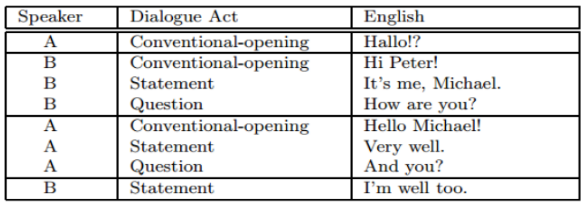
\includegraphics[width=10cm]{1.png}
\end{figure}

\section{Recurrent Neural Networks (RNN)}

Recurrent neural network is a type of artificial neural network. The problem of
remembering previous inputs to the network was solved by recurrent neural
networks with the help of hidden layers. Because of their internal memory, RNN
is able to remember important things about the input, which allows them to make
precise predictions about what’s coming next. This is why they are preferred
algorithm for sequential data. Sequential data is just ordered data where
related things follow each other.

\begin{figure}
	\caption{Recurrent vs Feed-forward Neural Network}
	\centering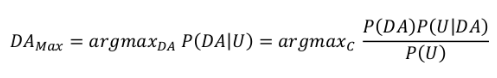
\includegraphics[width=10cm]{2.png}
\end{figure}

Unlike the normal feedforward neural networks, recurrent neural networks feed
the output of previous step to the current step. This helps the network to
memorise the previous inputs. So basically RNN cycles through the information,
i.e. when taking a decision it takes into consideration the current input as
well as whatever it learned from the previous output. For example, consider the
word ‘Teacher’, till the point a feed forward neural network reaches ‘c’ it
forgets about ‘t’, ‘e’ and ‘a’. A RNN remembers exactly that. Recurrent Neural
Network adds immediate past to the present. This is important since past data
contains information about what is coming next. 

RNN applies weight to current and also previous input and they tweak their
weights through gradient descent and backpropagation through time. Gradient
Descent is an algorithm that is used to iteratively minimize a given function.
Backpropagation Through Time (BPTT) is basically just a fancy buzz word for
doing Backpropagation on an unrolled Recurrent Neural Network. Unrolling is a
visualization and conceptual tool, which helps you to understand what’s going on
within the network. RNN can be viewed as a sequence of Neural Networks that is
trained one after another with backpropagation.

\begin{figure}
	\caption{Structure of a Neuron}
	\centering
\includegraphics[width=10cm]{3.png}
\end{figure}

The above diagram shows the RNN being unrolled after the equal sign. The
different timesteps are visualized and information gets passed from one timestep
to the next. Within BPTT the error is back-propagated from the last to the first
timestep, while unrolling all the timesteps. This allows calculating the error
for each timestep, which allows updating the weights.

\subsection{Problems with RNN}

\begin{enumerate}[align=left]

	\item Training RNNs is a difficult task.

	\item \textbf{Exploding gradient problem :} Exploding gradient is when
		the algorithm assigns a stupidly high importance to the weights,
		without much reason. But fortunately, this problem can be easily
		solved if you truncate or squash the gradients.

	\item \textbf{Vanishing gradient problem :} Vanishing gradient is when
		the values of a gradient are too small and the model stops
		learning or takes way too long because of that. This problem is
		solved by the concept of LSTM.

\end{enumerate}

\section{Long Short Term Memory}

Long Short Term Memory (LSTM) is an artificial recurrent neural network.
Consider LSTM as an extension to the recurrent neural network, which basically
extends its memory. Therefore they are capable of learning things that have very
large time lags between them. LSTM can remember this because they contain their
information in a memory, that is much like the memory of a computer because the
LSTM can read, write and delete information from its memory.

The memory in LSTM are gated cells. Gated cell means that he cell decides
whether or not to store or delete information based on the importance it assigns
to the information. The importance assigning takes place through weights which
are learned through the algorithm.

\begin{figure}
	\caption{Structure of a Basic LSTM node}
	\centering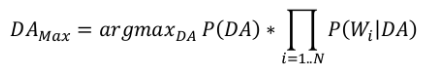
\includegraphics[width=10cm]{4.png}
\end{figure}

A basic LSTM node consists of input gate, output gate and forget gate. The input
gate decides whether or not to let new input in. The forget gate deletes the
information because it is not important. The output gate impacts the output at
the current time step. The gates in a LSTM are analog, in the form of sigmoids,
meaning that they range from 0 to 1. The fact that they are analog, enables them
to do backpropagation with it.

The problem of vanishing gradients which is very common in recurrent neural
networks is solved by LSTM as it keeps the gradient steep enough and therefore
the training short and the accuracy high.
	% Add each chapter here in this fashion.
				% No need to write all font and page specs in the chapter
				% files. There only typesetting tags are required.
%_____________________________________________________________________________________________ 
% LATEX Template: Department of Comp/IT BTech Project Reports
% Sample Chapter
% Sun Mar 27 10:25:35 IST 2011
%
% Note: Itemization, enumeration and other things not shown. A sample table is included.
%_____________________________________________________________________________________________ 

\chapter{Literature Survey}
\section{Automatic Cloze-Question Generation}
This paper describes a system that can generate a list of cloze questions from a
document. CQG system is divided into three main module - Sentence selection, Key
selection and Distractor selection. In the first stage, informative and relevant
sentences are selected from the document. In the second stage, keywords i.e the
words/phrases to be questioned on, are identified in the selected sentence. Key
selection will not be noun or adjective it would find on the basis of NER. The
first two stage are not domain specific. Distractors or answer alternatives for
the keyword in the question sentence are chosen in the final stage using web
scraping. third and final stage is made domain specific, as quality of
distractor depends on domain. 

\section{Automatic question generation on the basis of the discourse
connectives}

This paper describes a question generation system divided into two modules -
Content selection and Question formation. Content selection consists of finding
the relevant part in text to frame question form. The Question formation
involves several tasks like Sense disambiguation of the discourse connectives,
Identification of question type and Applying syntactic transformations on the
content. The authors have concentrated on seven discourse connectives like
because, since, although, as a result, for example and for instance. On that
basis the Question type will be decided using a rule based model. 

\section{Automatic Question Generation Using Software Agents for Technical
Institutions}

This paper explains a system which takes as input a text file and the output is
another text file containing questions. The system is based on Bloom’s taxonomy.
Bloom’s Taxonomy is a set of three hierarchical models used to classify
educational learning objectives into levels of complexity and specificity. The
three lists cover the learning objectives in cognitive, affective and sensory
domains. It has been proved that generating questions based on Bloom's taxonomy
accurately allows a teacher to judge the learning ability of the students. 

The proposed framework helps in question generation by deploying agents, which
perform various operations like Document Processing, Information Classification
and Question Generation. In Document processing phase stemming is carried out to
normalize the senses of the words. Information classification takes an list of
keyword generated by Document Processing and finds the Bloom's category of those
words, by searching appropriate action verb in the repository which fits with
the given keyword. Finally the Question generation module takes the output of
Information classification as input to generate questions. The process is a
template based approach, which fits the selected keywords in the question
template according to the Bloom's levels.

\section{Automatic Multiple Choice Question Generation System for Semantic
Attributes Using String Similarity Measures}

The paper describes a system which selects the informative sentence and the
keyword to generate a question on, based on the semantic labels and named
entities that exist in the sentence. The distractors are chosen based on a
similarity measure between sentences in the data set. For generating question
Semantic Role Labeler and Named Entity Recognizer is used to identify whether
its Name, Location or Name of Organization. Once a question is prepared, then it
measures the similarity between the ‘Question sentence’ and each of the
sentences from the Question knowledge. Then the obtained similarity values from
other sentences are sorted and three keywords from three different sentences are
obtained as distractor values.


\section{G-Asks: An Intelligent Automatic Question Generation System for
Academic Writing Support}

This paper describes a system generating specific trigger questions as a form of
support for student’s learning through writing. It describes a large-scale case
study, of 24 human supervisors and 33 research students, in an Engineering
Research Method course. It compares the questions generated by G-Asks with human
generated questions. The paper analyzes the most frequent question types,
derived from the human supervisors’ questions and discusses how the human
supervisors generate such questions from the source text.

\section{Semantic Based Automatic Question Generation}

This paper also describes a system that uses both Semantic Role Labeling and
Named Entity Recognizer technique to convert the inputted sentence to semantic
pattern. It has developed an Artificial immune system which classifies the
patterns according to the question type. The question types considered here are
the set of WH-questions. Immune system utilizes feature extraction, learning,
storage memory, and associative retrieval in order to solve recognition and
classification tasks. Inputted sentence will first parse using NER and SRL
technique, and from NER and SRL identifies whether, sentences contain person
name, location, date. On the basis of this identification, question pattern can
be created, i.e if person name then question pattern would be WHO.  Sentence
pattern for who and question patterns are interpreted as two features vector in
the training set, one vector for each question type.

\section{Automatic Generation Of Multiple Choice Questions From Domain
Ontologies}

This paper presents an approach that is based on domain specific ontologies and
it is independent of lexicons such as WordNet or other linguistic resources. The
model developed creates multiple choice question items using the Semantic Web
standard technology - Ontology Web Language. The proposed approach is
independent of the domain since questions are generated according to specific
ontology-based strategies. Class based, property based, terminology based
strategies were used to generate the questions. Property-based strategies are
described to produce a large number of multiple choice questions but are said to
be very difficult to manipulate syntactically. Class and terminology-based
strategies on the other hand are much easier to handle syntactically but
generate fewer questions for ontologies of the same depth and population.

\section{Mind the Gap: Learning to Choose Gaps for Question Generation}

In this paper the approach taken is that, the problem of generating good
questions is divided into two parts: First, the selection of sentences to ask
about, and Second, the identification of which part of the resulting sentences
the question should address. To achieve the goal of selecting better gap-fill
questions, author has broken down the task into multiple stages like Sentence
selection, Question construction, and eventually Classification and Scoring. For
generating question, features are used i.e. Token count, lexical, syntactic,
semantic and NER feature is used to generate the Gaps fill question.

\begin{center}
	\begin{longtable}{| p{0.6cm} | p{2.3cm} | p{4cm} | p{2cm} | p{5cm} |}
		\hline
		{\textbf{Sr No.}} & {\textbf{Algorithm}} & {\textbf{Methodology}} &
		{\textbf{Type of Question}} & {\textbf{Evaluation of Result}}\\[2ex]
		\hline
		1. &
		Cloze question generation &
		Sentence selection, key selection and distractor selection is
		domain specific and NER feature is used for key selection &
		Cloze &
		Manually Evaluation is done
		\begin{enumerate}[leftmargin=*]
		\item Evaluation of the selected sentence
		\item Evaluation of selected keyword 
		\item Evaluation of selected distractor.
		\end{enumerate}
		\\[1ex]
		\hline

		2. &
		Automatic question generation on the basis of the discourse
		connectives &
		Content selection and Question formation &
		Question generation like Why, when, where, in which &
		Manually evaluated for semantic and syntactic soundness of
		question by two evaluator
		\\[1ex]
		\hline
		3. &
		Automatic Question Generation Using Software Agents for
		Technical Institutions &
		Document Processing, Information Classification and Question
		Generation. &
		Define, Describes, Give example, long descriptive questions &
		-
		\\[1ex]
		\hline
		4. &
		G-Ask &
		Citation Extraction, Citation Classification. and Generation &
		Long descriptive questions like Why, when, Does any.. &
		Compared questions generated by the system to those produced by
		humans. and Citation Classification performance is done through
		precision and recall.
		\\[1ex]
		\hline
		5. &
		Automatic Multiple Choice Question Generation System &
		Extract sentence from Data Set, Prepare Question sentence,
		Measure the similarity between the question sentence and all
		sentences in the knowledge base, Return the three sentences that
		have the highest similarity values, three keywords of three
		sentences as distractor selection &
		MCQ &
		In this research out of nearly 145 parsed sentences, there were
		109 considered good according to the keywords that are extracted
		from them.
		\\[1ex]
		\hline
		6. &
		Semantic Based Automatic Question Generation &
		Input sentence, Feature Extraction through SRL, NER, Choose MCS,
		Test Sentence pattern and Test the Question type pattern &
		WH-questions like who, when, where, why, and how. &
		170 sentences are extracted and mapped into 250 patterns using
		SRL and NER. The 250 patterns are used in training and testing.
		and Precision, Recall and F-measurement is used for
		classification of question type.
		The percentage of truly generated patterns increased 87\% which
		appears to be promising ratio in this problem comparing it to
		other techniques used in generating questions automatically.
		\\[1ex]
		\hline
		7. &
		Automatic Generation of Multiple Choice Questions From Domain
		Ontologies &
		Ontology-based strategies like class based, property based,
		terminology based strategies &
		MCQ (Choose the correct sentence) &
		The generated questionnaires were evaluated in three dimensions:
		Pedagogical quality, linguistic/syntactical correctness and
		number of questions produced.
		\\[1ex]
		\hline
		8. &
		Mind the Gap: Learning to Choose Gaps for Question Generation &
		1)Sentence selection,
		2)Question construction,
		3)Classification/Scoring. &
		Fill in the blanks question &
		manually analyze the generated questions and rate the question
		\\[1ex]
		\hline
	\end{longtable}
\end{center}


%\begin{table}[H]		% Table
%\begin{center}		
%\begin{tabular}{ | c | c | }	% Format	
%\hline
%\multicolumn{2}{|c|}{Table 1: Test Century Records }\\
%\hline
%\bf{Batsman} & \bf{Test Centuries}\\ \hline
%Sachin & 51 \\ \hline
%Kallis & 40 \\ \hline
%Ponting & 39 \\ \hline
%Lara, Gavaskar & 34\\ 
%\hline
%\end{tabular}
%\caption{A simple table: Test centuries}	% This will appear in List of Tables
%\label{table1}
%\end{center}
%\end{table}

%_____________________________________________________________________________________________ 

		

\appendix
\chapter{Algorithm for Lighting}
\chapter{Flow Chart for Making Popcorn}

\bibliographystyle{plain}  % You can change the style of writing bibliography.
\bibliography{coep_compit_report} % Instead of a .bib file, you can just write it in 
				  % a text file with \bibitem entries.
%_____________________________________________________________________________________________ 
\end{document}			% End of Report

